% Typeset with XeTeX
% Allows use of system fonts rather than just LaTeX's ones
% NOTE - if you use TeXShop and Bibdesk (Mac), can complete citations
%  - open your .bib file, type~\citep{xx... and then F5 or Option-Escape
\documentclass[11pt]{article}
\usepackage[margin=1in, letterpaper]{geometry} % set page layout
%\geometry{letterpaper}  % or a4paper
\usepackage[xetex]{graphicx} % allows us to manipulate graphics.
% Replace option [] with pdftex if you don't use Xe(La)TeX
\usepackage{color}
\usepackage{indentfirst}
\usepackage{hyphenat}
\usepackage{epstopdf} % automatic conversion of eps to pdf 
\usepackage{amsmath, amssymb} % Better maths support & more symbols
\usepackage{textcomp} % provide lots of new symbols - see textcomp.pdf
% line spacing: \doublespacing, \onehalfspacing, \singlespacing
\usepackage{setspace}

\singlespacing
\usepackage{pgfplotstable}
% allows text flowing around figs
% use \begin{wrapfigure}{x}{width} where x = r(ight) or l(eft)
\usepackage{wrapfig}
\usepackage[parfill]{parskip} % don't indent new paragraphs
\usepackage{flafter}  % Don't place figs & tables before their definition 
\usepackage{verbatim} % allows \begin and \end{comment} regions
\usepackage{booktabs} % makes tables look good
\usepackage{bm}  % Define \bm{} to use bold math fonts
% linenumbers in L margin, start & end with \linenumbers \nolinenumbers,
\usepackage{lineno} % use option [modulo] for steps of 5
\usepackage[auth-sc]{authblk} % authors & institutions - see authblk.pdf
%\renewcommand\Authands{ and } % separates the last 2 authors in the list
% control how captions look; here, use small font and indent both margins by 20pt
\usepackage[small]{caption} 
\setlength{\captionmargin}{20pt}

%: FONT
% If you don't want to use system fonts, replace from here to 'Citation style' with \usepackage{Palatino} or similar
%: ************ FANCY FONTS START HERE
\usepackage[no-math]{fontspec} % 'no-math' = keep computer modern for math fonts
\usepackage{xunicode} % needed by XeTeX for handling all the system fonts nicely
\usepackage[no-sscript]{xltxtra} 
\setmonofont[Scale=0.8]{PT Serif} % typeface for \tt commands
\setsansfont[BoldFont={PT Serif Bold}, ItalicFont={PT Serif Italic}]{PT Serif} 
\defaultfontfeatures{Mapping=tex-text}
\setmainfont{Minion Pro}
%\setmainfont{Source Sans Pro}
%: ************ FANCY FONTS END HERE

%:CITATION STYLE
% natbib package: square,curly, angle(brackets)
% colon (default), comma (to separate multiple citations)
% authoryear (default),numbers (citations style)
% super (for superscripted numerical citations, as in Nature)
% sort (orders multiple cites into order of appearance in ref list, or year if authoryear)
% sort&compress: as sort, + multiple citations compressed (as 3-6, 15)
\usepackage[numbers,comma,sort&compress]{natbib}
\usepackage{nicefrac}
\usepackage{multirow}

%:SHORTCUT COMMANDS
% Maths
\newcommand{\ddt}[1]{\ensuremath{\frac{{\rm d}#1}{{\rm d}t}}}  % d/dt
\newcommand{\dd}[2]{\ensuremath{\frac{{\rm d}#1}{{\rm d}#2}}} % dy by dx  - \dd{y}{x}
\newcommand{\ddsq}[2]{\ensuremath{\frac{{\rm d}^2#1}{{\rm d}#2^2}}} % second deriv
\newcommand{\pp}[2]{\ensuremath{\frac{\partial #1}{\partial #2}}} % partial \pp{y}{x}
\newcommand{\ppsq}[2]{\ensuremath{\frac{\partial^2 #1}{\partial {#2}^2}}}
\newcommand{\superscript}[1]{\ensuremath{^{\textrm{#1}}}} %normal (non-math) font for super/subscripts in text
\newcommand{\subscript}[1]{\ensuremath{_{\textrm{#1}}}}
\newcommand{\positive}{\ensuremath{^+}}
\newcommand{\negative}{\ensuremath{^-}}
% Editing
\newcommand{\red}[1]{{\color{red}{#1}}}
\newcommand{\redtext}[1]{{\color{red}{#1}}}
\newcommand{\blue}[1]{{\color{blue}{#1}}}
\newcommand{\bluetext}[1]{{\color{blue}{#1}}}
\newcommand{\scinot}[2]{\ensuremath{#1 \times 10^{#2}}}
% Standard stuff
\newcommand{\be}{\begin{equation}}
\newcommand{\ee}{\end{equation}}
\newcommand{\bea}{\begin{eqnarray}}
\newcommand{\eea}{\end{eqnarray}}
\newcommand{\ie}{\textit{i.e.}}
\newcommand{\etal}{\textit{et al.}}
\newcommand{\khi}{Ki67$^\text{hi}$}
\newcommand{\klo}{Ki67$^\text{lo}$}


% \begin{graybox} text \end{graybox} for text with a background colour
\definecolor{MyGray}{rgb}{0.96,0.97,0.98}
\definecolor{MyGray}{rgb}{0.96,0.90,0.98}
\makeatletter\newenvironment{graybox}{%
	\begin{lrbox}
		{\@tempboxa}\begin{minipage}[r]{0.98\columnwidth}}{\end{minipage}\end{lrbox}%
	\colorbox{MyGray}{\usebox{\@tempboxa}}
}\makeatother


%%%%%%%%%%%%%%%%%%%%%%%

\title{Population dynamics of  B cell subsets -- analysis and predictions}
\author{}

\date{}

\begin{document} 
	\maketitle
	
	We aimed to quantify the dynamics of various subsets within mature B cell population and to understand the rules of replacement of old cells by that of new ones within each subset.
	%We adopted the conventional view of B cell development and assumed that Transitional 2 (T2) cells are the direct precursor of FM cells, which then participate in germinal centre (GC) reactions upon antigen interaction.
	We assumed that FM cells circulate freely in the lymphatic system, and so we pooled the numbers of these cells recovered from spleen and lymph nodes when modelling their dynamics.
	We compared different models of the population dynamics and structure of the FM compartment, as well as the possibilities that  the T1 or T2 transitional subsets may serve as their source population.
	In order to compare the time-varying chimerism in FM cells across animals with different levels of bone marrow chimerism and different sources, we normalised the FM chimerism to that in the common progenitor population,  \ie T1 cells.
	Here, we assess the suitability of T1, T2 and pooled (T1+T2) compartments as putative source populations for FM cells and explore various mechanisms that can explain their population dynamics in mice.
	
	
	%We define turnover to mean loss. 
	
	% In the busulfan chimeras, if the source is constant in time and all cells behave the same way, the existing population is replaced at rate $\lambda$, the net loss rate (turnover rate - division rate). 
	
	%So rate of replacement is not necessarily the rate of turnover (unless there is no division). Division compensates for turnover and keeps host cells in the pool for longer.
	
	%Might be worth coming up with a word for $\lambda$. I think 'clonal persistence --- low $\lambda$ means that a cell and its progeny survive for a long time (if $\lambda=0$, a clone persists for ever even though it may be dividing and dying; if $\lambda>0$, mean lifetime of a lineage (e.g. a cell and all its descendents) is $1/\lambda$. If $\lambda>0$, the cell population grows exponentially as $e^{\lambda t}$. 
	
	
	%\red{One concern: Sanket tried T1 as source and it actually gives better fits in all FM cases ($\Delta$LOO-ic $\simeq$ 5). But we are going with dogma and saying T2 is source. It's puzzling to us that there is apparently so much residual Ki67 expression in FM from the T2 source, if all the division is pre-T1 as you say. Makes me worry a littl...} 
	
	\section*{Follicular Mature B cells}
	
	\subsection*{Replacement kinetics are consistent with FM cells being a single, kinetically homogeneous population, with cell lifetime increasing with host age}
	The chimerism within the FM compartment stablised at the level of the upstream T1 precursors (i.e. normalised donor fraction $f_{d} \rightarrow 1$) by about 210d post-BMT, implying the near-complete replacement of the compartment within that timeframe. Complete replacement suggests that the average rates of loss across host and donor cell populations are always equal.
	Additionally, we measured the kinetics of their expression of Ki67, a nuclear protein expressed during cell cycle and lost with a lifetime of a few days following mitosis (Gossel eLife 2017 \red{and others - see refs in that paper}). Immediately following BMT the donor FM cells are highly enriched for recently divided cells, with around 80\% \khi, but this proportion falls slowly to equalise with that of host cells at around 10\% after approximately 100 days. \red{This kinetic is consistent with IDEA HERE}
	
	%We assumed a mean lifetime of Ki67 post-mitosis of 3.5d, and also assumed that \khi\ and \klo\ cells are lost at equal rates $\delta(t)$. The timecourses of host and donor \khi\ fractions were then generated by simulating the model with its best-fit parameters, beginning at the mean \khi\ fractions observed at 12d post-BMT, pooled across all experimental cohorts. See Methods below for details.}
	
	We modelled this behaviour by assuming that cells differentiate into FM B cells at a rate proportional to the their source population, and all FM cells, whether host or donor, are lost through death or differentiation  at rate $\delta$ and renewed through division  at rate $\rho$. For generality we allowed either of these rates to vary with the age of the host. We also considered the possibilities that the direct precursors of FM B cells are T1 cells, T2 cells, or T1 and T2 combined. We fitted each model  simultaneously to the timecourses of the total size, normalised donor chimerism normalised to T1 (the earliest common precursor to all populations considered) and the proportions of host and donor FM cells expressing Ki67 (Figure~\ref{fig:results_FM}A and B; see Methods for details). We found strongest support for T1 as the direct precursor of FM B cells, and the model in which the loss or turnover rate $\delta$ changes with host age and the division rate $\rho$ remains constant. Specifically, total numbers of FM B cells are given by
	\be
	\ddt{N_\text{FM}} = \;  \phi(t) + (\rho - \delta_{0}e^{-rt}) N_\text{FM},
	\label{eq:FM_total}
	\ee
	
	where $\phi(t)$ is the daily rate of influx from the source, whose kinetic was described empirically by fitting an empirical function to the timecourse of cell numbers. The data indicated the the size of the T1 and T2 populations  changed very little with host age and so these functions were nearly flat. Time is measured from age 40 days, at which time the loss rate is $\delta_{0}$. This model of time-dependent loss was superior to the simplest model with constant rates of division and turnover ($\Delta$LOO-ic = 8) and also superior to the alternative with a time-varying division rate ($\Delta$LOO-ic = 10). We estimate that FM B cells divide slowly, on average every 15 months,  and have a mean residence time of $\sim$34 days in 7 week-old mice. This life expectancy doubles on an average every $\sim$28 months.
	We also predict that approximately 4\% of FM B cells are replaced each day by newly differentiated cells from the T1 population. Parameter estimates and 95\% confidence intervals are in Table 2.
	
	We also define the net loss rate $\lambda$ as the aggregate of cell division and turnover (i.e. $\delta - \rho$), which decreases with time for FM cells, as $\delta$ declines.
	This suggests that in old animals individual FM clones and their progeny would persist longer in follicles than in younger animals, purely due to gradual increase in their survival.
	%Even with the low levels of proliferation seen in FM cells longer-lived clones are possible because of increase in survival rate of cells and their progeny.
	
	\subsection*{No evidence for  heterogeneity within FM B cells}
	
	The decline we detect in $\lambda$ with host age, %which we infer derives from progressively increased survival within the FM compartment,
	therefore drives a gradual slowing of the approach to stable chimerism relative to the kinetic predicted by a simple model of constant division and turnover. An alternative explanation of this time-varying kinetic is that the FM pool comprises independent sub-populations with different but constant rates of division and turnover, each fed from the T1 source.  In this scenario, less persistent populations (those with a high net loss rate $\lambda$) will be replaced most rapidly after BMT, giving an initial steep upslope in chimerism. There will then follow a slower increase as the more persistent FM subpopulations (with low $\lambda$) are replaced by donor cells relatively slowly.
	
	We fitted a model of kinetic heterogeneity assuming two independent subpopulations, allowing their relative size and their constant loss rates ($\delta_{1}$ and $\delta_{2}$) and division rates ($\rho_{1}$ and $\rho_{2}$)  to be free parameters. However this model received lower support than the model of FM cells as a single population with turnover slowing with host age ($\Delta$LOO-ic = 7, Table \ref{tab:FM-AICs}).   Indeed there was a very weak signature of kinetic heterogeneity;  the estimated loss and division rates of the two FM subpopulations were nearly equal  ($\delta_{1}$ = 0.38 (0.02, 1.1), $\delta_{2}$ = 0.21 (0.01, 0.99), $\rho_{1}$ = 0.10 (0.001, 0.72), $\rho_{2}$ = 0.18 (0.0002, 0.63)). % and close to that of the simplest homogeneous model with $\lambda$ = 0.029 (0.024, 0.033).
	
	We also found no evidence for any host-donor differences in kinetics in the form of a persistent host-derived `incumbent' population (Table~1). For the discussion of the Incumbent model, see methods [Hogan et al. PNAS 2015 Rane et al. PLoS Biology 2018].
	Another potential mechanism for slowing replacement with host age is a decline in the rate of influx (e.g. a fall in the rate of differentiation from T2) with host age. We found no evidence for this ($\Delta$LOO-ic = 18), hence rejected the possibility.
	
	\begin{figure}[h!]
		\centerline{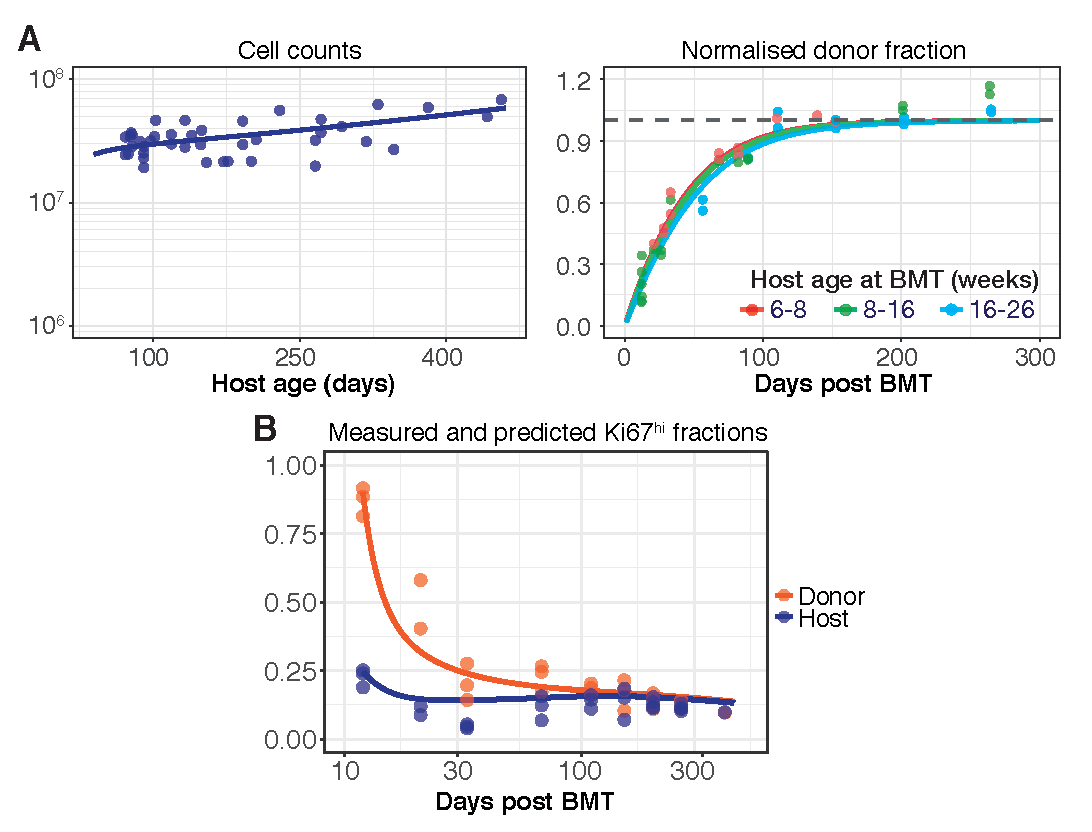
\includegraphics[scale = 0.85] {Results_FM.pdf}}
		\caption{\small \textbf{Fitted and predicted   population dynamics of FM B cells, using the best-fitting model in which cells divide at a constant rate and their mean residence time increases with host age.}  The model was fitted simultaneously to the extended timecourses of total cell counts of FM B cells pooled from LN and spleen in busulfan chimeras, the donor fractions in FM B cells normalised to the chimerism in T1 cells and the proportion of cells that were \khi\ within host and donor FM B cells. Solid lines denote the most probable description of the observations of (A) cell counts, (B) normalised donor fractions and (C) \khi fractions using the time-dependent model with envelopes indicating uncertainty in the model fit. Prediction intervals (4.5$^{th}$ and 95.5$^{th}$ percentiles) were plotted by drawing samples from the posterior distribution of parameter estimates. Different colours in (A) and (B) indicate the different groups of hosts, binned according to the age at which they were transplanted with donor BM cells. Model predictions for individual groups were drawn using the mean age at BMT.}
		\label{fig:results_FM}
	\end{figure}
	
	%\subsection*{The model of time-varying loss successfully predicts the kinetics of Ki67 expression within host and donor populations}
	%As well as the numbers of host and donor-derived cells in the FM compartment, we  also measured the kinetics of their expression of Ki67, a nuclear protein expressed during cell cycle and lost with a lifetime of 3-4 days following mitosis (Gossel eLife 2017 \red{and others - see refs in that paper}). Immediately following BMT the donor FM cells are highly enriched for recently divided cells, with around 80\% \khi, but this proportion falls slowly to equalise with that of host cells at around 10\% after approximately 100 days (Figure~\ref{fig:results_FM}C, red and green points).
	
	%As a validation of the models,  which were fitted only to the timecourses of total FM B cell numbers and chimerism, we used them to predict the dynamics of Ki67 expression within host and donor cells over time. The best-fitting time-dependent homogeneous model  predicted these kinetics remarkably well. These predictions were generated by inserting the estimated rates of loss ($\delta(t) = \delta_{0} e^{-rt}$) and division ($\rho$) into a model which explicitly follows the transit of cells between \khi\ and \klo\ states, which we have employed previously (Hogan PNAS 2015, Gossel eLife 2017). We assumed a mean lifetime of Ki67 post-mitosis of 3.5d, and also assumed that \khi\ and \klo\ cells are lost at equal rates $\delta(t)$. The timecourses of host and donor \khi\ fractions were then generated by simulating the model with its best-fit parameters, beginning at the mean \khi\ fractions observed at 12d post-BMT, pooled across all experimental cohorts. See Methods below for details.
	
	%The simulations show that the host/donor disparity in Ki67 expression derives largely from residual expression of Ki67 on cells that have recently entered the FM pool from the T2 precursor population \red{T2s are not dividing, you say... so surely this is further evidence that T1s are the source for FMs?}.  Soon after BMT, the donor FM pool is highly enriched for these recent immigrants, roughly 80\% of which are Ki67,  relative to the more established host-derived pool. The lifetime of FM cells is relatively short and so a substantial fraction of newly immigrated \khi\ cells  are lost before they transition to \klo. This interplay means that quiescent donor cells are slow to accumulate. In parallel, Ki67 levels transiently dip in host FM cells following BMT due to the sudden reduction in influx from the host T2 pool, before they re-establish equilibrium at lower numbers. 
	
	\subsection*{Summary}
	\begin{itemize}
		\item Most support for model in which FM B cell residence time increases with host age
		\item No evidence for kinetic heterogeneity (\ie\ multiple subpopulations with different turnover, or host incumbents) 
		%\item No evidence for changes in the per-cell rate of differentiation from T2 with cell age
		\item No evidence for changes in rates of loss or division of FM cells with cell age.
	\end{itemize}
	
	%of \khi\ fractions within host and donor compartments .
	%The possible explanation for this is that majority of ki67 in FM compartment is source derived suggesting that FM cells are primarily maintained by high influx from source and by very low levels of cell division.
	%The high influx corresponds to high loss rate (inverse of residence time, Table~\ref{tab:FM-parestm}) in the FM subset, which only allows for slow accumulation of \klo\ cells post BMT in the donor compartment. 
	%Inflow of very high (> 90\% of donor influx) numbers of \khi\ cells with gradual accrual of \klo\ population, temporarily maintains high fractions of \khi\ cells within donor compartment, which slowly stabilise to levels equivalent to that of the host compartment as donor fractions stabilise.
	%In the host compartment, since pre-existing cells are mostly \klo, the low inflow ($\chi \sim$ 0.8)  of new \khi\ cells doesnt alter the kinetics of \khi\ fractions within these cells.
	%In summary, we find no strong evidence for heterogeneity within FM B cells which are suggested to be firmly regulated by the homeostatic factors changing with the age of the host.
	
	%: Table 1
	\begin{table}[h!]
		\begin{center}
			\renewcommand{\arraystretch}{1.25}
			\begin{tabular}{c c c c c} 
				\toprule 
				\multicolumn{4}{c}{\textbf{Model and $\Delta$Loo-ic}} \\
				\cline{2-5}
				Source &{\small Time-dependent}  & {\small Simple homogeneous} &  {\small Kinetic heterogeneity} & {\small Incumbent} \\ 
				\toprule
				T1      &   0             &              8             &                7              &          9         \\ 
				T2      &   36            &              43            &                39             &          42        \\ 
				T1 + T2 &   19            &              29            &                28             &          29        \\ 
				\hline
				\toprule 
			\end{tabular}
		\end{center}
		\caption{\small \textbf{Comparison of models describing population dynamics of Follicular Mature (FM) B cells, pooled from LN and spleen}. Loo-ic values obtained using leave-one-out cross validation method are shown relative to that of the best fitting model, in which the rate of loss  (turnover) of FM cells declines slowly with the age of the host. Predictions of more complex models were very close to those of the simple homogenous model (that is, either very little kinetic heterogeneity, close to zero incumbent cells, or effects of cells age on turnover or division rates)}. 
		\label{tab:FM-AICs}
	\end{table} 
	
	\vspace{1cm}
	
	
	%: Table 2
	\begin{table}[h!]
		\begin{center}
			\renewcommand{\arraystretch}{1.25}
			\begin{tabular}{ l r l } 
				\toprule 
				\textbf{Parameter}  &  {\small Estimate}  &  {\small 95\%  $^{\ast}$CI} \\ 
				\toprule
				Percent daily replacement by source at age 7 wks          & 3.9      &  (3.2, 13)  \\
				Mean clonal lifetime (days) at age 7 wks                  & 38       &  (30, 48)  \\
				Mean residence time (days) at age 7 wks                   & 34       &  (26, 42)  \\ 
				Mean inter-division time (days)                           & 268      &  (120, 1600)  \\
				Time for mean residence time to double (months)           & 28       &  (15, 180)  \\
				Average time of loss of Ki67 expression (days)            & 6.0      &  (4.6, 7.3)  \\
				\hline
				\toprule 
			\end{tabular}
		\end{center}
		\caption{\small \textbf{Parameter estimates from the best-fit (Time-dependent) model using T1 compartment as the source population for FM B cells (Spleen + LN)}. $^{\ast}$Credible intervals were estimated by taking 2.5$^{th}$ and 97.5$^{th}$ percentiles of the posterior probability distribution of the parameter values obtained after fitting model to the data.}
		\label{tab:FM-parestm}
	\end{table} 
	
	\clearpage
	
	\section*{Germinal Center B cells}
	
	\subsection*{Invasion kinetics of donor-derived GC cells differ between spleen and lymph nodes.}
	To explain the replacement  kinetics of GC cells in busulfan chimeric mice, we used diverse models that address the heterogeneity in GC compartment and test the effects of host-age on their dynamics (described above in FM section and in Methods).
	All models were fitted simultaneously to an extensive time-course of total counts, donor fractions ($f_{d}$) and the proportions of \khi cells that spans over a year.
	The donor fractions in Spleen and LN GC compartments were normalised to the donor fractions in the common progenitor population, \ie T1 cells, so as to compare them across animals with different levels of bone marrow chimerism.
	This also allows us to explore the suitability of splenic T1 and the pools of T2 and FM cells that circulate freely between spleen and LN as the putative source populations for spleen and LN GC cells. 
	
	Our data shows that the normalised $f_{d}$ in splenic GC cells stabilises twice as fast as their lymph node counterparts ($\sim$110 and $\sim$260 days post BMT for spleen and LN GCs, respectively), suggesting a strong disparity in the invasion kinetics of donor cells between these two pools. 
	Additionally, we found that recently divided YFP-tagged splenic GC cells were lost twice as fast as LN GC cells in Ki67-CreER-YFP reporter mice (half life 11 vs 20 days respectively, details in the Methods?).
	Due to such differences observed in the population dynamics of spleen and LN GC cells, we decided to model them separately.
	We assumed a constant rate of source influx in both spleen and LN GC pools and allowed our models to be strongly informed by the rate of turnover ($\lambda$) observed in Ki67-CreER-YFP reporter mice.
	
	
	%: Table 1
	\begin{table}[h!]
		\begin{center}
			\renewcommand{\arraystretch}{1.25}
			\begin{tabular}{l l c c c c} 
				\toprule 
				&         & \multicolumn{4}{c}{\textbf{Model and $\Delta$Loo-ic}} \\
				\cline{3-6}
				\textbf{Population} & Source     & {\small Simple homogeneous}&  {\small Time-dependent}    & {\small Kinetic heterogeneity} & {\small Incumbent} \\ 
				\toprule
				SPGC &   T1    &   17           &          9            &           33         &          12        \\ 
				     &   T2    &   10           &          0            &           33         &          9         \\ 
				     &   FM    &   13           &          8            &           32         &          9         \\ 
				\hline
				LNGC &   T1    &   55           &          41           &           12         &          54        \\ 
				     &   T2    &   50           &          42           &           12         &          51        \\ 
				     &   FM    &   12           &          35           &           0          &          38        \\ 
				\hline
				\toprule 
			\end{tabular}
		\end{center}
		\caption{\small \textbf{Comparison of models describing population dynamics of GC B cells}. Loo-ic values obtained using leave-one-out cross validation method are shown relative to that of the best fitting model. We consider $\Delta$Loo-ic values $\ge$6 of statistical significance for model selection.} 
		\label{tab:GC-AICs}
	\end{table} 
	
	\subsection*{The population dynamics of spleen GC cells are influenced by the age of the host.}
	We find that the total numbers of spleen GC cells increase over time but the proportions of \khi cells remain constant and almost identical between donor and host cells (Figure~\ref{fig:results_SPGC}).
	These results suggest that there is either a substantial increase is the size of the source population or a decline in the turnover of spleen GC cells with host-age.  
	As observed earlier, the size of FM subset increases over time, but their chimerism changes more slowly and stabilises much later (at $\sim$210 days post BMT) than in spleen GCs, suggesting that transitional (T1 and/or T2) subsets are more likely candidates for the source population. 
	Indeed, we found that the model of time-varying loss (where the net loss rate $\lambda$ declines with host-age) using T2 as the source of spleen GCs, received strongest statistical support ~(Table~\ref{tab:GC-AICs}) and produced best visual descriptions of the trends in total cell counts, normalised $f_{d}$ and proportions of \khi cells in splenic GC cells (Figure~\ref{fig:results_SPGC}). 
	
	Our analysis shows that rapidly dying spleen GC clones are sustained for about 15 days by equally rapid division rate in 7w old mice (Table~\ref{tab:SPGC-parestm}).
	The ability of B cell clones to persist in splenic GC pool increases as animals get older due to a relative increase in their residence time $(\nicefrac{1}{\delta})$ in spleen, which doubles every $\sim$8 months.
	Models in which the rate of source influx or the inter-division time of GC cells varies with host-age produced poorer fits and received inferior statistical support  ($\Delta$Loo-ic $\ge 8$).  
	We also find that the maintenance of spleen GC compartment is mainly dependent on the source influx as a fairly large proportion of GC cells in spleen ($\sim$ 36\% of total counts in 7w old mice) are daily replaced by the cells from the circulatory pool of T2 compartment. 
	%The time-dependent model with T2 as the source has the fairly large probability (Akaike weight 94\%) to predict new information as compared to all the other models and sources explored in this analysis. 
	
% Table 2
\begin{table}[h!]
\begin{center}
		\renewcommand{\arraystretch}{1.25}
		\begin{tabular}{l l }
			\toprule
			\textbf{Parameter}                                & \textbf{Estimates and 95\% CI} \\
			\toprule
			%Akaike weight (\% )                                     & 94                   \\
			Source influx $(\# \text{of cells} \times 10^{-3})$      & 4.7 (3.2, 6.8)       \\
			Mean clonal lifespan `$\tau$' at 7w of host age (days)   & 15 (13, 16)           \\
			Mean resident time at 7w of host age  (days)             & 0.46 (0.34, 0.61)     \\			
			Mean inter-division time (days)                          & 0.48 (0.35, 0.64)     \\
			Time taken for $\tau$ to double(months)                  & 7.9 (4.5, 25)        \\
			Average time of loss of Ki67 expression (days)           & 5.2 (3.8, 6.7)  \\					
			\hline
			\toprule 
		\end{tabular}
	\end{center}
	\caption{\small \textbf{Parameter estimates from the best-fit (Time-dependent) model using T2 compartment as the source population for SP GC B cells.}  Credible intervals were estimated by taking 2.5$^{th}$ and 97.5$^{th}$ percentiles of the posterior probability distribution of the parameter values obtained after fitting model to the data.}
	\label{tab:SPGC-parestm}
\end{table} 
	
\subsection*{Lymph node GC population contains the mixture of transient and persistent clones.}
The GC compartment in lymph nodes shows a modest increase in its size over time with steady and high proportions of \khi cells that are almost identical between host and donor sub-populations (Figure \ref{fig:results_LNGC}C), very similar to what observed in the spleen.
We found that the models with assumptions of homogeneity within the GC compartment failed to capture the trend in total cell numbers and slow stabilisation of the normalised $f_{d}$, even after allowing host-age dependent alterations in their turnover. 
The replacement kinetics of LN GC cells were best explained by the model that assumes kinetically distinct subsets within GC population, as reflected by its visual descriptions of the trends in cell counts, normalised $f_{d}$ and fractions of \khi cells in LN GC compartment (Figure~\ref{fig:results_LNGC}) and superior statistical support (Table~\ref{tab:GC-AICs}). 
Our data also identified FM compartment as the most likely source of LN GCs as compared to T1 and T2 Transitional subsets ($\Delta$Loo-ic $\ge$ 12, Table~\ref{tab:GC-AICs}).
%Fits from the kinetic heterogeneity model to the time-course  of using FM compartment as the source population are shown in .

Our analysis reveals that some GC clones are extremely short-lived and are cleared from the lymph nodes within days (average clonal lifespan of $\sim$ 5days, Table~\ref{tab:LNGC-parestm}) while others can persist for as long as 2 months (Table~\ref{tab:LNGC-parestm}).
The presence of pre-existing host-derived `persistent' GC clones  may explain the slow replacement kinetics of GC compartment in lymph nodes.
In a 7 week old mouse, the LN GC compartment is equally divided between `transient' and persistent clones and we speculate that this ratio would skew towards latter in older animals.
The accumulation of persistent clones over time may also explain the gradual increases in the pool size of LN GC cells.
We also find that roughly 25\% LN GC cells are replaced daily by the new cells entering from the pool of FM cells that are freely circulating between spleen and LN.


%: Table 3
\begin{table}[h!]
	\begin{center}
		\renewcommand{\arraystretch}{1.25}
		\begin{tabular}{l l l }
			\toprule
			\multirow{2}{*}\textbf{Parameter}                 & \multicolumn{2}{l}{\textbf{Estimates and 95\% CI}} \\
			                                                  & \small{Transient Subset}  & \small{Persistent Subset} \\
			\toprule
			%Akaike weight                                         &\multicolumn{2}{c}{99} \\         
			Source influx $(\# \text{of cells} \times 10^{-2})$    & 7.0 (0.2, 40)        & 24 (12, 43)  \\
			Mean clonal lifespan (days)                            & 5.0 (1.2, 19)        & 68 (34, 130)  \\
			mean resident time   (days)                            & 0.69 (0.42, 1.3)     & 0.90 (0.46, 1.9)  \\				
			mean inter-division time (days)                        & 0.91 (0.47, 2.0)     & 0.79 (0.46, 1.9)  \\
			Fraction of total population at 7w of host age         & 0.51 (0.17, 0.72)    & 0.49 (0.28, 0.83)    \\	
			Average time of loss of Ki67 expression (days)         & 5.1 (3.7, 6.6)       & 5.1 (3.7, 6.6)      \\	
			\hline
			\toprule 
		\end{tabular}
	\end{center}
	\caption{\small \textbf{Parameter estimates from the best-fit (Kinetic heterogeneity) model using FM compartment as the source population for LN GC B cells.}  Credible intervals were estimated by taking 2.5$^{th}$ and 97.5$^{th}$ percentiles of the posterior probability distribution of the parameter values obtained after fitting model to the data.}
	\label{tab:LNGC-parestm}
\end{table} 
	
	\begin{figure}[h!]
		\centerline{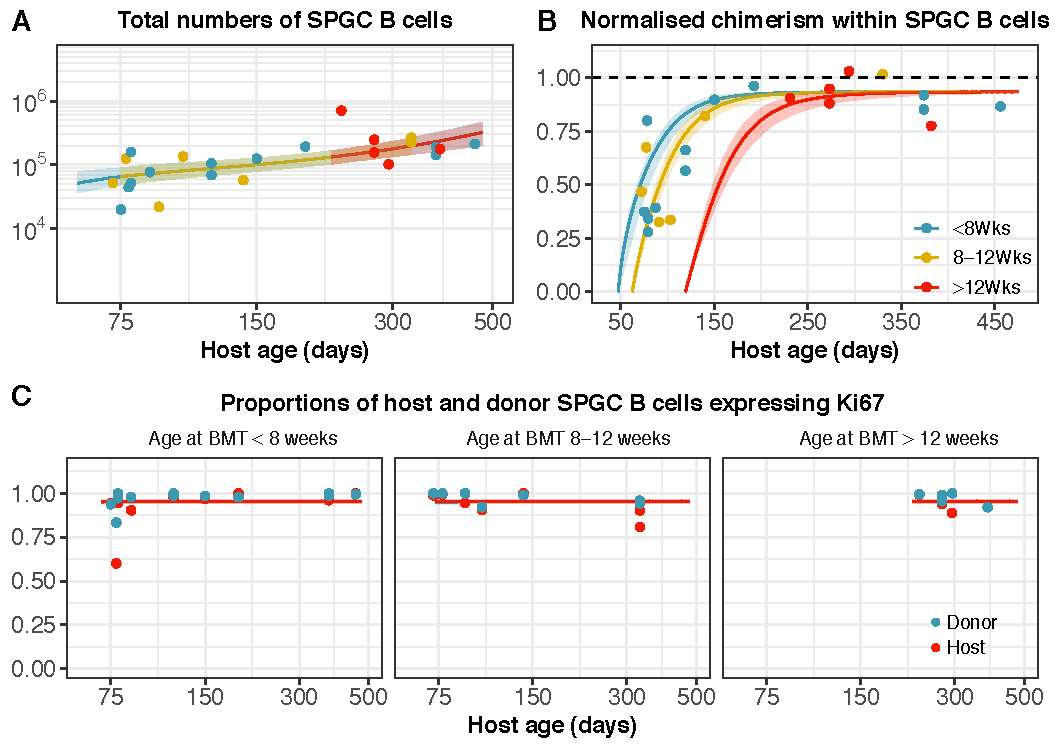
\includegraphics[scale = 0.85] {Results_SPGC_T2.pdf}}
		\caption{\small \textbf{Fitted and predicted population dynamics of spleen GC B cells, using the best-fitting Time-dependent model with T2 as the source.}  The model was fitted simultaneously to the time-course of total cell counts of spleen GC B cells, the donor fractions normalised to the chimerism in T1 cells and the proportions of \khi cells within their host and donor compartments. The time-dependent model fit to the time-course of normalised $f_{d}$ stabilises at a value <1, precisely equal to the ratio of donor fraction in T2 to the donor fraction in T1. Solid lines denote the most probable description of the observations of (A) cell counts, (B) normalised donor fractions and (C) \khi fractions using the time-dependent model with envelopes indicating uncertainty in the model fit. Prediction intervals (4.5$^{th}$ and 95.5$^{th}$ percentiles) were plotted by drawing samples from the posterior distribution of parameter estimates. Different colours in (A) and (B) indicate the different groups of hosts, binned according to the age at which they were transplanted with donor BM cells. Model predictions for individual groups were drawn using the mean age at BMT.}
		\label{fig:results_SPGC}
	\end{figure}
    
    
    \begin{figure}[h!]
    	\centerline{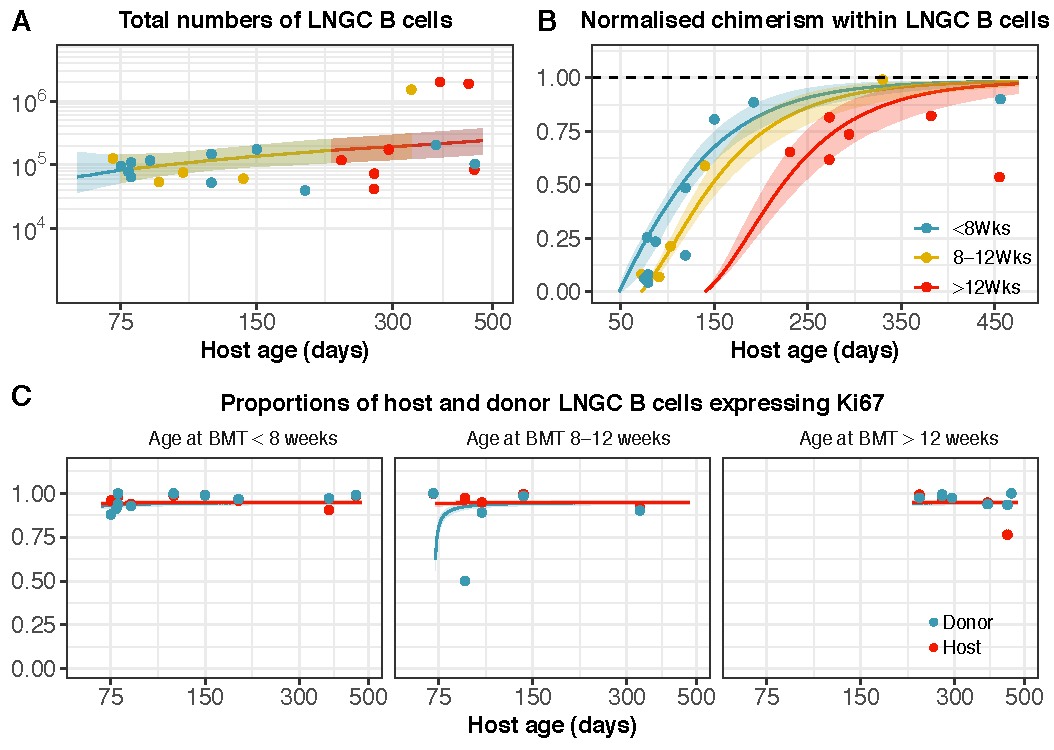
\includegraphics[scale = 0.85] {Results_LNGC_FM.pdf}}
    		\caption{\small \textbf{Fitted and predicted population dynamics of LN GC B cells, using the best-fitting Kinetic heterogeneity model with FM as the source.}  The model was fitted simultaneously to the  time-course of total cell counts of GC B cells pooled from multiple lymph nodes of busulfan chimeric mice, the donor fractions normalised to the chimerism in T1 cells and the proportions of \khi cells within their host and donor compartments.  The kinetic heterogeneity model fit to the time-course of normalised $f_{d}$  approaches 1, following the trend in donor fraction in FM normalised to the donor fraction in T1. Solid lines denote the most probable description of the observations of (A) cell counts, (B) normalised donor fractions and (C) \khi fractions using the time-dependent model with envelopes indicating uncertainty in the model fit. Prediction intervals (4.5$^{th}$ and 95.5$^{th}$ percentiles) were plotted by drawing samples from the posterior distribution of parameter estimates. Different colours in (A) and (B) indicate the different groups of hosts, binned according to the age at which they were transplanted with donor BM cells. Model predictions for individual groups were drawn using the mean age at BMT.}
    		\label{fig:results_LNGC}
    \end{figure}
	

	\subsection*{Discussion}
	\begin{itemize}
		\item GC cell dynamics vary between spleen and lymph nodes, as observed by slower replacement kinetics of LN GC cells  as compared to their splenic counterparts.
		Accordingly, our analysis predicts longer persistence of a large fraction of GC cells in lymph nodes than in spleen.
		
		\item Heterogeneity in LNGCs stems from pooling multiple LNs?
		
		\item Prolong GC reactions in response to viral antigens and gut microbes (Adachi et al. 2015, Bachman et al. 1996, Kasturi et al. 2011) may allow B cells to reach higher degree of affinity maturation $\rightarrow$ means to cope with constant antigenic drifts. 
		An important question is whether chronic GC response consists of long-lived GC cells or constant invasion of short lived cells maintaining a long-lived steady state?
		
		\item Ki67 in GC is result of active division and turnover and is not source derived. FM population has 10\% \khi cells while GC are $\sim$ 95\% \khi. 
	\end{itemize}
	

	
\end{document}




